\subsection{Study Area}



The study area for this research is Janaki Rural Municipality, located in Nepalgunj, Banke District, Nepal (Figure\ref{fig:study_area_map}). Situated at an elevation of 165m above sea level, it is bordered by Nepalgunj Sub-Metropolitan City to the east, Kohalpur Municipality to the north, Khajura Rural Municipality to the west, and the international boundary with India to the south (Janaki Rural Municipality). The region features a temperate climate and flat terrain. Meteorological records indicate an average annual rainfall of 1445.58~mm, with temperatures ranging from a minimum of 4.5°C to a maximum of 46°C (Janaki Rural Municipality).
\begin{figure}[H]
    \centering
    \caption{Study Area: Janaki Rural Municipality, Banke, Nepal} 
    \label{fig:study_area_map}
    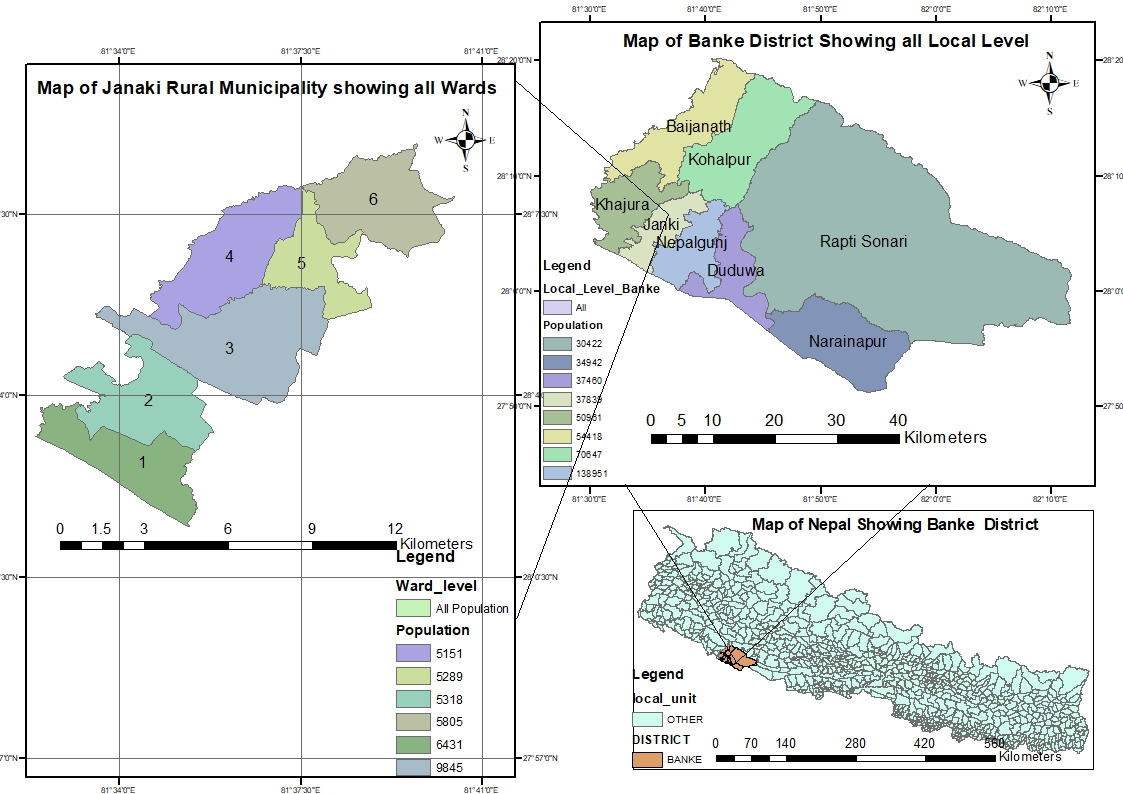
\includegraphics[width=0.9\textwidth]{images/study_area_map.png}
\end{figure}

Agriculture is the primary livelihood for most households in Janaki Rural Municipality. Of the 5,063ha of cultivable land, only 2,532ha are utilized, comprising 1,798ha of farmland and 774ha of upland. Land ownership varies widely: 1,294 households possess less than 0.167ha, 1,222 hold 0.2--0.33ha, 2,338 own 0.37--0.67ha, 1,512 control 0.7--1ha, and 973 own more than 20ha, while 52 households are landless (Janaki Rural Municipality, 2075). Irrigation remains limited, with only 321ha irrigated year-round and 1,871~ha lacking consistent water access. The municipality contains 50 ponds, some of which support irrigation. Despite abundant arable land, inadequate irrigation and limited technological resources hinder commercial agriculture, resulting in dependence on food imports from India (Janaki Rural Municipality, 2075).
    
Janaki Rural Municipality is divided into six wards, of which three were randomly selected for this study (Table~\ref{tab:study_area}). 

\begin{table}[ht]
\centering
\caption{Study Area with elevation and coordinates}
\label{tab:study_area}
\resizebox{\textwidth}{!}{
\begin{tabular}{|c|l|c|l|}
\hline
\textbf{S.N.} & \textbf{Study Location} & \textbf{Elevation (m)} & \textbf{Coordinates} \\ \hline
1 & Janaki Rural Municipality – 01, Saigaun & 164 & 28°02'42"N 81°34'05"E \\ \hline
2 & Janaki Rural Municipality – 03, Indrapur & 172 & 28°05'02"N 81°36'20"E \\ \hline
3 & Janaki Rural Municipality – 04, Khajura Khurda & 163 & 28°06'26"N 81°36'00"E \\ \hline
\end{tabular}
}
\end{table}

Source: (Janaki Rural Municipality, 2075)

\subsubsection{Methods of Data Collection}
\paragraph{Primary Data Sources}
A comprehensive household survey and intensive field research were conducted across wards 1, 3, and 4 of Janaki Rural Municipality, encompassing 47 villages. Structured interviews and direct observations were employed to gather data on agricultural practices, irrigation access, food security, and perceptions of climate change. Village sample sizes were determined based on household ratios derived from municipal records, followed by systematic sampling of households within each village to ensure representativeness.
\paragraph{Secondary Data Sources}
Secondary data were sourced from a literature review pertinent to the research objectives. Desk-based research, primarily utilizing online resources, provided the majority of the data. Additional information was obtained from reference books, recently published national newspapers, peer-reviewed international journals, government reports, historical records, and relevant websites.
\subsubsection{Sampling Frame}
The study employed stratified random sampling to select wards 1, 3, and 4 from the six wards of Janaki Rural Municipality, using a lottery method for ward selection. These wards were chosen to represent the municipality’s diversity, with ward 1 comprising 5 villages and wards 3 and 4 each containing 21 villages, as documented in an internal survey from 2075 B.S. Villages within each ward were sampled proportionally using stratified random sampling to enhance diversity and reduce sampling bias. Households within selected villages were then systematically chosen based on household data provided by the municipality. Field observations complemented the survey by providing additional insights into household conditions and local agricultural practices.

Details of the household distribution across the sampled wards are presented in Table~\ref{tab:household_distribution}. The table summarizes the number of households from wards 1, 3, and 4 of Janaki Rural Municipality, providing a foundation for the study’s analysis of agricultural and environmental conditions.

\begin{table}[h]
\centering
\caption{Household Distribution by Ward in Janaki Rural Municipality}
\label{tab:household_distribution}

\begin{tabular}{|c|c|c|}
\hline
\textbf{Ward} & \textbf{Household}  \\ \hline
1 & 1242  \\ \hline
3 & 1929  \\ \hline
4 & 1050 \\ \hline
\textbf{Total} & 7391 \\ \hline
\end{tabular}
\end{table}

\subsection{Sample Size Determination}  
The total household population was derived from an internal survey conducted by Janaki Rural Municipality in 2075 B.S. (Janaki Rural Municipality). The sample size for the questionnaire survey was calculated at a 95\% confidence level using the following formula (Dahal 2021):

\[
n = \frac{N \cdot z^2 \cdot p \cdot q}{(N - 1) \cdot e^2 + z^2 \cdot p \cdot q}
\]

where:
\begin{itemize}
    \item $n$ = sample size,
    \item $N$ = total number of households in selected wards (4,221),
    \item $z$ = z-score for 95\% confidence level (1.96),
    \item $p$ = expected prevalence (0.9),
    \item $q$ = $1 - p$ (0.1),
    \item $e$ = margin of error (0.05).
\end{itemize}

Substituting the values:

\[
n = \frac{4221 \cdot (1.96)^2 \cdot 0.9 \cdot 0.1}{(4221 - 1) \cdot (0.05)^2 + (1.96)^2 \cdot 0.9 \cdot 0.1} = 133.9 \approx 134
\]

The sample size for each ward ($n_h$) was determined proportionally using the formula (Dahal 2021)

\[
n_h = \frac{N_h}{N} \cdot n
\]

where:
\begin{itemize}
    \item $n_h$ = sample size per ward,
    \item $N_h$ = number of households in the ward,
    \item $N$ = total household population (4,221),
    \item $n$ = total sample size (134).
\end{itemize}

\subsection{Sample Size of Selected Wards}  
The proportional sample sizes for wards 1, 3, and 4 are presented in Table~\ref{tab:sample_size_wards}.


\begin{table}[h]
\centering
\caption{Sample Size of Selected Wards in Janaki Rural Municipality}
\label{tab:sample_size_wards}
\begin{tabular}{|c|c|c|c|}
\hline
\textbf{Ward} & \textbf{$N_h$} & \textbf{$N_h / N$} & \textbf{$N_h / N \cdot n$} \\ \hline
1 & 1242 & 0.29 & 39 \\ \hline
3 & 1929 & 0.457 & 61 \\ \hline
4 & 1050 & 0.249 & 33 \\ \hline
\textbf{Total} & 4221 & & 134 \\ \hline
\end{tabular}
\end{table}

\subsubsection{Data Collection and Calculation}  
This study aimed to examine production trends, climatic scenarios, and their interrelationships within the research area. Data collection involved integrating primary, secondary, and ancillary sources to ensure a robust and comprehensive analysis. Primary data were gathered through household surveys and field observations in Janaki Rural Municipality, as detailed in earlier sections. Secondary data were sourced from government reports, academic literature, books, and reputable organizations, including the Department of Hydrology and Meteorology (DHM) and the Ministry of Agriculture and Livestock Development (MOALD). Ancillary data from credible websites enhanced the dataset’s timeliness and depth. This multifaceted approach ensured the reliability, richness, and contextual relevance of the data. Statistical analyses were performed using IBM SPSS Statistics (version 27) and Microsoft Excel.

\paragraph{Pearson Correlation Coefficient}  
The Pearson correlation coefficient ($r$) was calculated to assess the linear relationship between crop yield (dependent variable) and climatic factors---sunshine hours, accumulated rainfall, and average temperature (independent variables)---prior to regression analysis. This coefficient, ranging from -1 to 1, quantifies the strength and direction of linear associations. A value of $r = 1$ indicates a perfect positive correlation, $r = -1$ a perfect negative correlation, and $r = 0$ no linear correlation. The formula is:

\[
r = \frac{n \sum_{i=1}^{n} (x_i - \bar{x})(y_i - \bar{y})}{\sqrt{\sum_{i=1}^{n} (x_i - \bar{x})^2} \sqrt{\sum_{i=1}^{n} (y_i - \bar{y})^2}}
\]

where $x_i$ and $y_i$ are individual data points, $\bar{x}$ and $\bar{y}$ are the means of variables $X$ and $Y$, and $n$ is the number of observations.

\paragraph{Simple Linear Regression Analysis}  
Simple linear regression was employed to model the relationship between crop yield ($Y_i$, dependent variable) and individual climatic variables ($X_i$, independent variables). This method estimates the linear effect of an independent variable on the dependent variable. The regression equation is:

\[
Y_i = \beta_0 + \beta_1 X_i + \epsilon
\]

where $\beta_0$ is the intercept, $\beta_1$ is the slope, and $\epsilon$ is the error term capturing unexplained variation.

\paragraph{T-test}
A two-sample t-test was conducted to compare average crop yields (kg/ha) between plots with year-round irrigation and those reliant on rainfed irrigation during the monsoon season. Year-round irrigation refers to plots with consistent water supply, while rainfed irrigation depends solely on seasonal rainfall. The null hypothesis $(H_0) $posits no difference in yields between groups, against the alternative $(H_1)$ of a significant difference. The significance level was set at $\alpha = 0.05$, and analysis was performed in SPSS.
The t-test statistic is:

\[
t = \frac{\overline{x_1} - \overline{x_2}}{\sqrt{s^2 \left( \frac{1}{n_1} + \frac{1}{n_2} \right)}}
\]

where $\overline{x_1}$ and $\overline{x_2}$ are group means, $s^2$ is the pooled variance, and $n_1$ and $n_2$ are sample sizes.

\paragraph{Index Model}  
An index model was developed to assign index values to unit areas, facilitating the creation of a ranking map. Similar to binary models, it employs overlay operations and multicriteria assessment but generates continuous index scores rather than binary outcomes.
The process involved two stages:

(1) assigning weights to variables based on relative importance, 

(2) scoring observed values.

\paragraph{Climate Change and Production Trend Analysis}  
Simple linear regression, implemented in IBM SPSS Statistics (version 27), was used to model the relationship between crop yield (dependent variable) and climatic variables---accumulated precipitation, average temperature, and sunshine radiation (independent variables). Pearson correlation coefficients were first calculated to assess linear associations, followed by regression analysis to quantify trends over time. This dual approach provided insights into both the strength and direction of relationships between yield and climate factors.

\paragraph{Climate Change Trends}  
Three climatic variables---accumulated rainfall, average temperature, and sunshine hours---were analyzed over a 30-year period (1990--2021) in the study area. Data were sourced from the Department of Hydrology and Meteorology (DHM). Linear trends were visualized using Microsoft Excel, with graphs illustrating changes in each variable over time.

\paragraph{Climate Change Perception}  
An index model evaluated farmers’ perceptions of climate change and its impact on agricultural production, recognizing that such perceptions shape adaptation strategies. A survey of 134 respondents assessed opinions on climate change using a three-point scale: +1 for agreement/approval, -1 for disagreement/disapproval, and 0 for “don’t know/absent.” For binary variables, the perception index was calculated using the formula by \parencite{dahalNutrientManagementSustainability2021}:

\[
\text{INDEX} = \frac{FA(+1) + FDA(-1) + FDK(0)}{N}
\]

where:
\begin{itemize}
    \item $FA$ = frequency of agreement/approval,
    \item $FDA$ = frequency of disagreement/disapproval,
    \item $FDK$ = frequency of “don’t know/absent,”
    \item $N$ = total respondents (134).
\end{itemize}

For variables with multiple categories, a normalized index was computed based on \parencite{nguyenduycanAssessingLivelihoodVulnerability2019}:

\[
\text{INDEX} = \frac{(\text{Max value} - \text{Min value}) \times X}{(\text{Max value} + \text{Min value}) \times \text{Max value}}
\]

where $X$ is the observed value of a specific category, and Max/Min values define the range of responses.
